\documentclass[12pt,onecolumn]{article}

\usepackage{listings}
\usepackage{float}
\usepackage{mathtools}
\usepackage[russian]{babel}
\everymath{\displaystyle}
\usepackage{color}
\usepackage{listings} 
\usepackage[usenames]{color}
\usepackage{placeins}
\usepackage{geometry}
\geometry{
  a4paper,
  top=25mm, 
  right=15mm, 
  bottom=25mm, 
  left=15mm
}

\begin{document}
\setcounter{tocdepth}{4}
\begin{center}
    Санкт-Петербургский Национальный Исследовательский\\ 
    Университет ИТМО\\
    Факультет Программной Инженерии и Компьютерной Техники\\
    
\includegraphics[scale=0.3]{itm.jpg} % нужно закинуть картинку логтипа в папку с отчетом
\end{center}
\vspace{1cm}


\begin{center}
    \large \textbf{Вариант №1610}\\
    \textbf{Лабораторная работа №1}\\
    по дисциплине\\
    \textbf{'Основы профессиональной деятельности'}
\end{center}

\vspace{2cm}

\begin{flushright}
  Выполнил Студент  группы number\\
  \textbf{Student's name}\\
  Преподаватель: \\
  \textbf{Teacher's name}\\
\end{flushright}

\vspace{6cm}
\begin{center}
    г. Санкт-Петербург\\
    2021г.
\end{center}

\newpage
\tableofcontents
\newpage

\section{Пункт 1}
\subsection{Создать приведенное в варианте дерево каталогов и файлов с содержимым. В качестве корня дерева использовать каталог lab0 своего домашнего каталога. Для создания и навигации по дереву использовать команды: mkdir, echo, cat, touch, ls, pwd, cd, more, cp, rm, rmdir, mv}
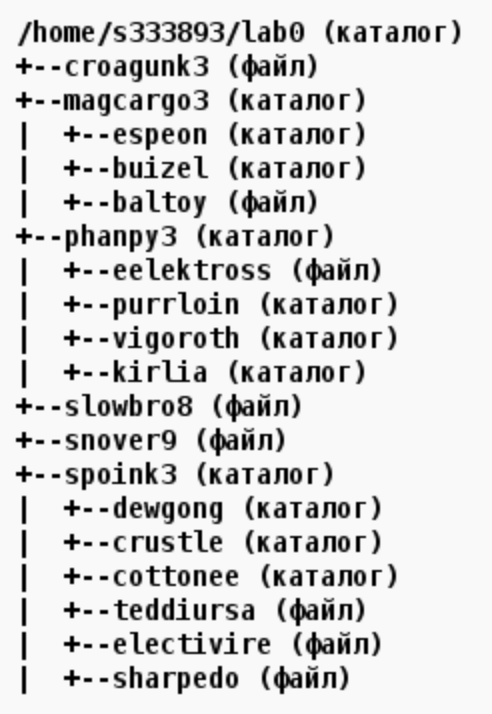
\includegraphics[scale=0.7]{p1.png}
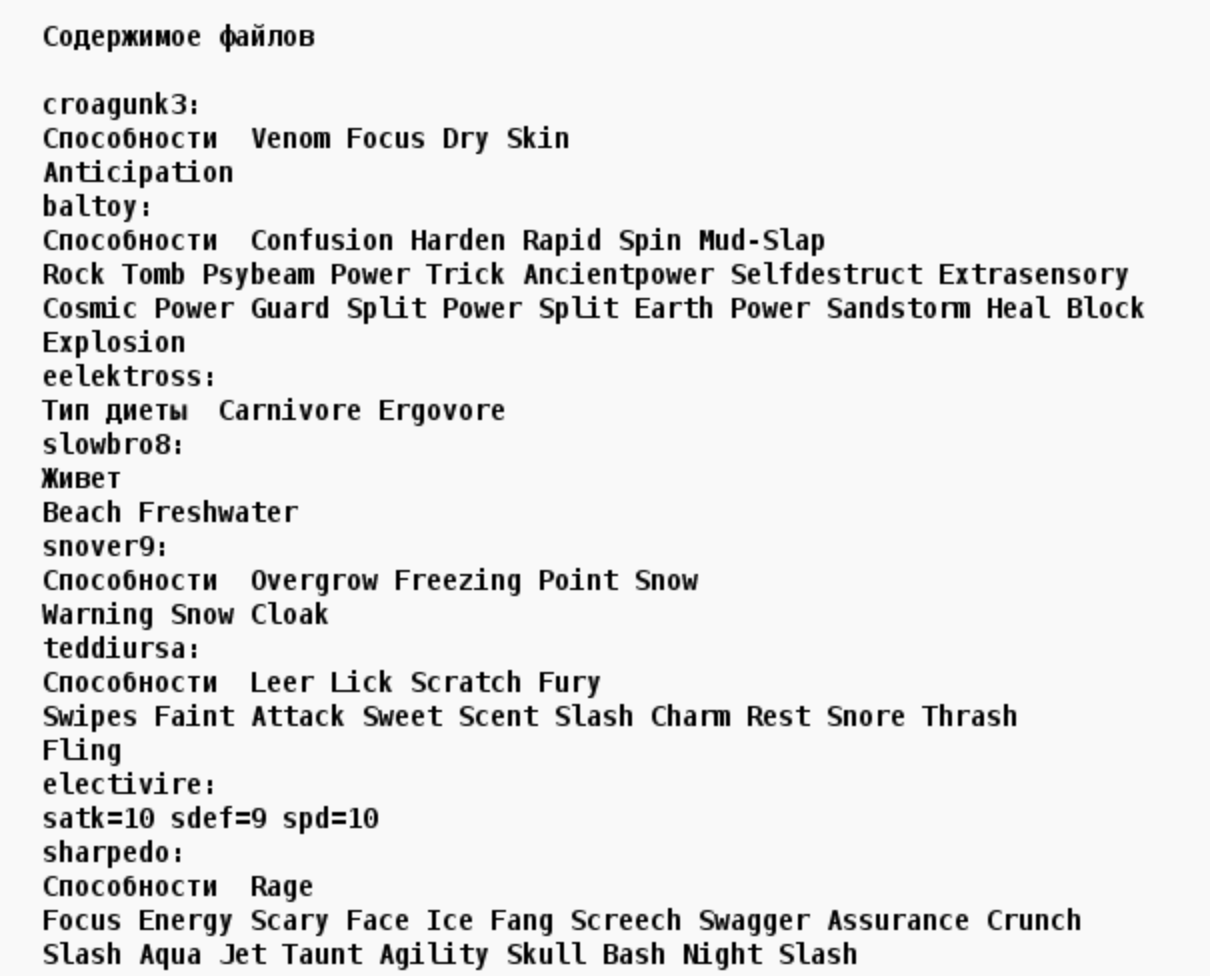
\includegraphics[scale=0.5]{p1-2.png}
\paragraph{Команды:}\\
\hfill\\
\lstloadlanguages{bash}
\definecolor{mygray}{RGB}{120,120,120}
\lstset{extendedchars =/true,
breaklines=true,
basicstyle=\ttfamily\fontsize{9pt}{9pt}\selectfont,
commentstyle=\color{mygray}}
\lstinputlisting[language=bash,numbers=left]{code1.sh}
\section{Пункт 2}
\subsection{Установить согласно заданию права на файлы и каталоги при помощи команды chmod, используя различные способы указания прав.}
\begin{itemize}  
\item croagunk3: владелец должен не иметь никаких прав; группа-владелец должна не иметь никаких прав; остальные пользователи должны читать файл
\item magcargo3: -wx-wx-wx
\item espeon: владелец должен записывать директорию и переходить в нее; группа-владелец должна читать и записывать директорию; остальные пользователи должны только переходить в директорию
\item buizel: r-x--x-wx
\item baltoy: владелец должен читать файл; группа-владелец должна не иметь никаких прав; остальные пользователи должны читать файл
\item phanpy3: -wxrwxr-x
\item eelektross: ------rw-
\item purrloin: rwxrw-r--
\item vigoroth: владелец должен читать, записывать директорию и переходить в нее; группа-владелец должна записывать директорию и переходить в нее; остальные пользователи должны записывать директорию и переходить в нее
\item kirlia: владелец должен читать директорию и переходить в нее; группа-владелец должна только переходить в директорию; остальные пользователи должны записывать директорию
\item slowbro8: владелец должен не иметь никаких прав; группа-владелец должна читать файл; остальные пользователи должны читать и записывать файл
\item snover9: права 644
\item spoink3: права 330
\item dewgong: права 305
\item crustle: rwxr-x-w-
\item cottonee: права 750
\item teddiursa: владелец должен не иметь никаких прав; группа-владелец должна читать и записывать файл; остальные пользователи должны не иметь никаких прав
\item electivire: права 444
\item sharpedo: r--------
\end{itemize}
\begin{center}
\paragraph{Команды:}\\
\hfill\\
\lstloadlanguages{bash}
\definecolor{mygray}{RGB}{120,120,120}
\lstset{extendedchars =/true,
breaklines=true,
basicstyle=\ttfamily\fontsize{9pt}{9pt}\selectfont,
commentstyle=\color{mygray}}
\lstinputlisting[language=bash,numbers=left]{set_permissions.sh}
\end{center}
\section{Пункт 3}
\subsection{Задание: Скопировать часть дерева и создать ссылки внутри дерева согласно заданию при помощи команд cp и ln, а также комманды cat и перенаправления ввода-вывода.}

\subsubsection{Объеденить содержимое файлов lab0/spoink3/electivire, lab0/spoink3/teddiursa, в новый файл lab0/croagunk3\_80}

\paragraph{Команды:}

cat spoink3/electivire spoink3/teddiursa >> croagunk3\_80

\subsubsection{Скопировать содержимое файла croagunk3 в новый файл\\ lab0/spoink3/teddiursacroagunk}

\paragraph{Команды:}

cat croagunk3 >> spoink3/teddiursacroagunk 
\subsubsection {Создать жесткую ссылку для файла slowbro8 с именем\\
lab0/spoink3/sharpedoslowbro}
\paragraph{Команды:}
ln slowbro8 spoink3/sharpedoslowbro
\subsubsection {Создать символическую ссылку c именем Copy\_6 на директорию spoink3 в каталоге lab0}\\

\paragraph{Команды:}\\
ln -s spoink3 Copy\_6

\subsubsection {Скопировать рекурсивно директорию phanpy3 в директорию\\ lab0/magcargo3/buizel}\\

\paragraph{Команды:}\\

cp -R phanpy3 magcargo3/buizel

\subsubsection {Скопировать файл croagunk3 в директорию lab0/magcargo3/espeon}\\

\paragraph{Команды:}\\

cp croagunk3 magcargo3/espeon

\subsubsection{Создать символическую ссылку для файла slowbro8 с именем\\ lab0/spoink3/sharpedoslowbro}\\

\paragraph{Команды:}\\
ln -fs \$(pwd)/slowbro8 \$(pwd)/spoink3/sharpedoslowbro\\
\paragraph{Иерархия файлов и каталогов, полученная при помощи команд ls -lR из директории lab0, после выполнения п.3 задания:}.
\begin{lstlisting}      
lrwxr-xr-x   1 aleksejlapin  staff    7  6 окт 11:16 Copy_6 -> spoink3
-------r--   1 aleksejlapin  staff   57  6 окт 11:16 croagunk3
-rw-r--r--   1 aleksejlapin  staff  136  6 окт 11:16 croagunk3_80
d-wx-wx-wx   5 aleksejlapin  staff  160  6 окт 11:16 magcargo3
d-wxrwxr-x   6 aleksejlapin  staff  192  6 окт 11:16 phanpy3
----r--rw-   1 aleksejlapin  staff   28  6 окт 11:16 slowbro8
-rw-r--r--   1 aleksejlapin  staff   71  6 окт 11:16 snover9
d-wx-wx---  10 aleksejlapin  staff  320  6 окт 11:16 spoink3
lab0/magcargo3:
ls: magcargo3: Permission denied

lab0/phanpy3:
ls: phanpy3: Permission denied

lab0/spoink3:
ls: spoink3: Permission denied
\end{lstlisting}

\section{Пункт 4}
\subsection{Задание: Используя команды cat, wc, ls, head, tail, echo, sort, grep выполнить в соответствии с вариантом задания поиск и фильтрацию файлов, каталогов и содержащихся в них данных.}
\subsubsection{Рекурсивно подсчитать количество строк содержимого файлов из директории lab0, имя которых начинается на 's', отсортировать вывод по увеличению количества, подавить вывод ошибок доступа}
\paragraph{Команды:}
wc -l \$(ls -R 2 > /dev/null  | grep \^ \large s) 2> /dev/null | sort -k 1n | grep -v "total" \large 2 > /dev/null
\paragraph{Результат выполнения:}
2 snover9
\subsubsection{Вывести четыре последних элемента рекурсивного списка имен и атрибутов файлов в директории lab0, список отсортировать по убыванию даты модификации файла, ошибки доступа не подавлять и не перенаправлять}
\paragraph{Команды:}\\
ls -ltR | tail -4

\paragraph{Результат выполнения: }
\hfill\\
ls: spoink3: Permission denied\\
ls: phanpy3: Permission denied\\
ls: magcargo3: Permission denied\\
./phanpy3:\\
./magcargo3:\\

\subsubsection{Рекурсивно вывести содержимое файлов из директории lab0, имя которых начинается на 's', строки отсортировать по имени z->a, добавить вывод ошибок доступа в стандартный поток вывода}
\paragraph{Команды:}\\
ls -R | grep \^ \large s | sort -r 2>\&1
\paragraph{Результат выполнения: }
\hfill\\
ls: magcargo3: Permission denied\\
ls: phanpy3: Permission denied\\
ls: spoink3: Permission denied\\
spoink3\\
snover9\\
slowbro8\\

\subsubsection{Вывести список имен файлов в директории phanpy3, список отсортировать по имени $a \rightarrow z$, ошибки доступа не подавлять и не перенаправлять}
\paragraph{Команды:}
ls phanpy3 | sort
\paragraph{Результат выполнения: }
\hfill\\
ls: phanpy3: Permission denied
\subsubsection{Подсчитать количество символов содержимого файлов в директории phanpy3, отсортировать вывод по увеличению количества, ошибки доступа не подавлять и не перенаправлять}
\paragraph{Команды:}
wc -m phanpy3/\$(ls phanpy3)
\paragraph{Результат выполнения: }
\hfill\\
ls: phanpy3: Permission denied\\
wc: phanpy3/: open: Permission denied\\
\subsubsection{Вывести содержимое файлов в директории phanpy3, исключить строки, заканчивающиеся на 'h', добавить вывод ошибок доступа в стандартный поток вывода}
\paragraph{Команды:}
\hfill\\
ls phanpy3 > > trash~ \&\&~ rm trash \&\&~ grep -v  "h\$" \, \$(ls~ -d \$(pwd)/phanpy3/*) 2>\&1
\paragraph{Результат выполнения: }
\hfill\\
ls: phanpy3: Permission denied
\section{Пункт 5}
\subsection{Выполнить удаление файлов и каталогов при помощи команд rm и rmdir согласно варианту задания.}
\subsubsection{Удалить файл slowbro8}
\paragraph{Команды:}
\hfill\\
rm slowbro8
\paragraph{Результат выполнения: }
\hfill\\
rm: slowbro8: override protection 46 (да/нет)?
\paragraph{Команды, исправляющие ошибки}
\hfill\\
chmod u+w slowbro8\\
rm slowbro8\\
\subsubsection{Удалить файл lab0/spoink3/sharpedo}
\paragraph{Команды:}
\hfill\\
rm spoink3/sharpedo
\paragraph{Результат выполнения: }
\hfill\\
rm: spoink3/sharpedo: override protection 400 (да/нет)?
\paragraph{Команды, исправляющие ошибки}
\hfill\\
chmod u+w spoink3/sharpedo\\
rm spoink3/sharpedo\\
\subsubsection{Удалить символические ссылки lab0/spoink3/sharpedoslowbro}

\paragraph{Команды:}
\hfill\\
rm spoink3/sharpedoslowbro

\subsubsection{Удалить жесткие ссылки lab0/spoink3/sharpedoslowbro}
\paragraph{Команды:}
\hfill\\
rm spoink3/sharpedoslowbro
\paragraph{Результат выполнения: }
\hfill\\
rm: spoink3/sharpedoslowbro: No such file or directory
\paragraph{Команды, исправляющие ошибки}
\hfill\\
Не называть жескую и символичускую ссылку одинаковым именем или ложить их в разные директории.
\subsubsection{Удалить директорию magcargo3}
\paragraph{Команды:}
\hfill\\
rmdir magcargo3
\paragraph{Результат выполнения: }
\hfill\\
rmdir: magcargo3: Directory not empty
\paragraph{Команды, исправляющие ошибки}
\hfill\\
chmod -R 777 magcargo3\\
rm -R magcargo3\\
\subsubsection{Удалить директорию lab0/phanpy3/kirlia}
\paragraph{Команды:}
\hfill\\
rmdir phanpy3/kirlia
\section{Вывод}
В этой лабораторной работе я научился работать с:
\begin{itemize}
\item Основными командами UNIX 
\item Правами доступа и файловой системой
\item Потоками данных
\item Символическими и жёсткими ссылками
\end{itemize}
\section{Cписок литературы}
\begin{thebibliography}{0}
\bibitem {Linux и UNIX программирование в shell}
«Linux and UNIX Shell Programming» --- David Tansley
\end{thebibliography}
\end{document}